
Leisure travelling is an impactful industry
whose economic importance significantly improves each
year, contributing to 10.4\% of the global GDP in 2019
~\cite{wttc2018travel}. Despite this, planning for a trip to a
foreign city requires a substantial amount of
time-consuming research. As a result, people often
rely on multiple data sources such as travel
brochures, blogs and vlogs to form a holiday plan and
retrieve the top-rated points of interests (POI) of a site. 
However,  these mediums do not hold the
resources to provide POIs tailored according to the traveller's preferences ,and
constraints and a tourist has to compile a timetable
independently
~\cite{DeChoudhury2010}. 

In literature, offering tourists a personalised route
composed of POIs has been defined as the tourist trip
design problem (TTDP). The TTDP comprises ranking
and selecting POIs that might interest the user and
create a feasible plan. 
This is an NP-hard problem where complete 
algorithms only manage to optimise with a small number
of POIs. Therefore, many approximate algorithms,
namely heuristic and meta-heuristic approaches, work
to converge solutions with complex alternatives to
this problem.

Nevertheless, the few existing systems that provide
users with an itinerary or activity plan require a lengthy
process of manually gathering the users' likes and
constraints or information from past trips. 
\\
\\

\noindent  We will try to answer the following research question:


\begin{center}

\textit{Can a system automatically recognise a tourist's travel
preferences and use this information to generate a personalised itinerary
for a holiday?}

\end{center}


%\begin{figure}[h]
%\centering
%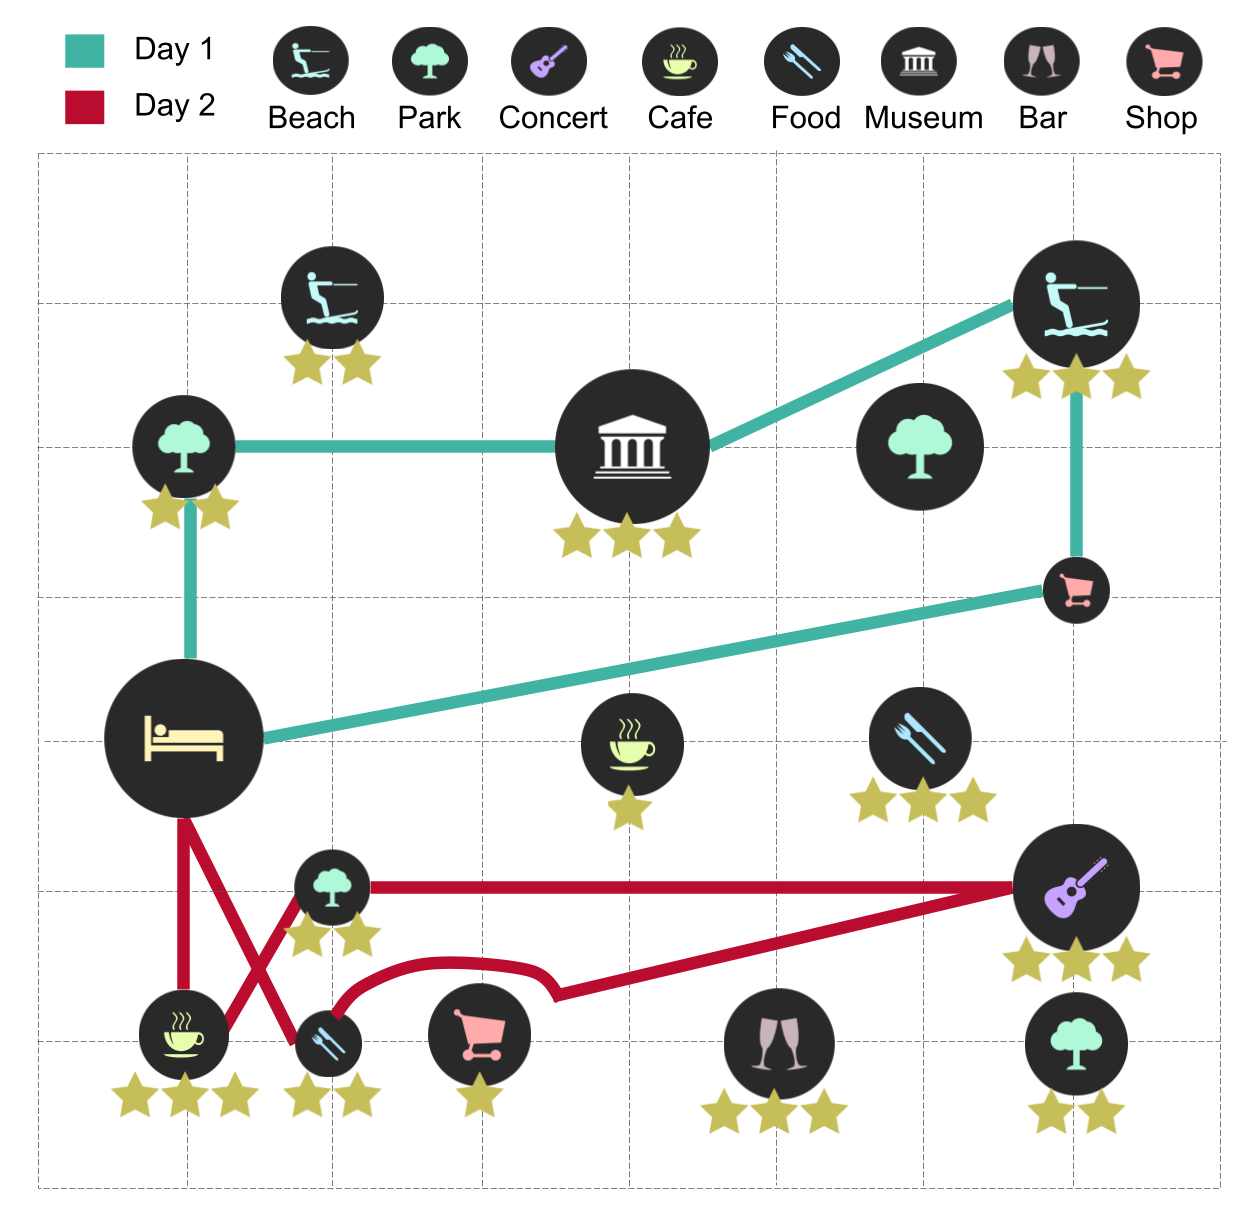
\includegraphics[width=0.4\textwidth]{TTDP.png}
%\caption{Example of a tourist planning problem}
%\label{TTDP}
%\end{figure}
